\documentclass[a4paper, french, 11pt, draft]{article}
\usepackage[utf8]{inputenc}
\usepackage[T1]{fontenc}
\usepackage[margin = 1.5 cm]{geometry}
\usepackage{graphicx}
\graphicspath{./images/}
\usepackage{amsmath}
\usepackage{tcolorbox}
\usepackage{minted}
\usepackage{animate}
\usepackage[backend=biber, citestyle=numeric-comp, bibstyle=numeric]{biblatex}
%\addbibresource{citations.bib}
\usepackage{csquotes}
\bibliography{citations.bib}

\usepackage{babel}

\newcommand{\nuance}[1]{\og #1 \fg}
\renewcommand{\emph}[1]{\textbf{#1}}

\title{Rapport simulation}
\author{Yves Abraham, Victoire Célarier, Eliott Chomard}
\date{25 novembre 2021}

\begin{document}
    \maketitle
    \section*{Introduction}
    Expérimentalement, il est apparu qu'une exposition de l'acier à l'hydrogène peut le fragiliser. Il serait donc intéressant d'accéder à la concentration en hydrogène dans le matériaux afin de comprendre où la fragilisation sera la plus importante. 
    Seules des méthodes de simulation permettent \og d'accéder \fg à ces données. Elles présentent aussi l'avantage d'évaluer l'influence de certains paramètres comme la concentration initiale ou la déformation imposée sur le processus de diffusion de l'hydrogène dans le matériau de manière plus aisée que des méthodes expérimentales.
    Ces simulations ont pu avoir une valeur "prédictive" au cours de notre MIG vis à vis de résultats expérimentaux qui arrivaient en différé, nous aurons l'occasion d'y revenir.
    Nous avons réalisé ces simulations avec le logiciel Zebulon -développé par le centre des matériaux- qui s'appuie sur la méthode des éléments finis.

    Cette simulation suppose de connaître la loi de comportement (équation qui lie contrainte et déformation) des matériaux considérés (X70 et X52). Nous avons donc commencé par déterminer empiriquement les lois de comportements des matériaux utilisés à partir d'éprouvettes \nuance{standards}. Dans un second temps, nous avons utilisé ces lois pour simuler le comportement d'éprouvettes \nuance{entaillées}.

    Une des idées à retenir de notre travail est que la concentration en hydrogène va être maximale où la pression est maximale. Dans l'idée de faire circuler de l'hydrogène dans des réseaux \nuance{vieillissants} de canalisations en acier, ce résultat questionne la faisabilité d'un tel projet; les zones les plus sollicitées dans le matériaux le seront d'autant plus du fait de la détérioration causée par l'hydrogène.

    Nos simulations ne rendent pas compte de la détérioration des caractéristiques mécaniques des matériaux, mais seulement de la dynamique de diffusion de l'hydrogène.

    \section{Étude du matériau}
    \subsection{Hypothèses générales de simulation}

    \begin{figure}[hbt]
        \animategraphics[width=0.6\textwidth, autoplay, loop, controls]{5}{image/effets_3D/MOVIE/step_}{000}{010}
        \centering
        \caption{Effet des différentes hypothèses sur le résultat}
        \label{anim:effet_3D}
    \end{figure}

    \subsection{Identification de la loi de comportement}
    Afin de modéliser le comportement d'un matériau, on se doit de l'étudier dans des cas simples, avant d'extrapoler son comportement dans des cas plus complexes.
    C'est pourquoi, nous avons commencé par étudier la réponse des aciers X52 et X70, taillé dans une éprouvette normalisée (de type SST), avant de la réutiliser dans le cadre de la simulation de la diffusion de l'hydrogène.
    La fonction d'écrouissage recherchée est la relation entre l'allongement et les contraintes, internes et mesurables, du matériau.
    En effet, une fois que l'acier est contraint au-delà de sa limite d'élasticité (ce n'est plus le réseau cristallin seul qui se déforme), une \og forêt \fg de dislocation se développe au sein du matériau, empêchant de plus amples dislocations de se former, augmentant ainsi la résistance du matériau.
    On supposera que cette loi est indépendante de la géométrie du matériau, isotrope, homogène, intrinsèque et invariante pour l'acier étudié.
    En observant la courbe de traction expérimentale, on donne une forme aux lois d'écrouissage du type:
    \begin{itemize}
        \item Pour l'acier X70:
        \[
            \sigma(\epsilon) = R0 + Q_1e^{-b_1\epsilon} + Q_2e^{-b_2\epsilon}
        \]
        \item Pour l'acier X52:
        \[
            \sigma(\epsilon) = \max(M + D\epsilon, R0 + Qe^{b\epsilon} + H\epsilon)
        \]  
    \end{itemize}
    Pour obtenir les bons coefficients pour la relation, il s'agit de comparer les courbes expérimentales et simulées, pour différents jeux de paramètres. 
    Une des particularités de l'identification au centre des matériaux est l'utilisation de données supplémentaires, que sont la mesure tout au long de l'essai de la contraction diamétrale de l'éprouvette.
    Cette mesure permet d'avoir accès à la section vraie en tout temps, et d'obtenir un modèle fiable même après que l'éprouvette ait commencé à strictionner.
    On peut voir en figure \ref{fig:X52_fit} et \ref{fig:X70_fit} les résultats des simulations sur les aciers X70 et X52, sur une éprouvette de type SST.

    \begin{figure}[ht]
        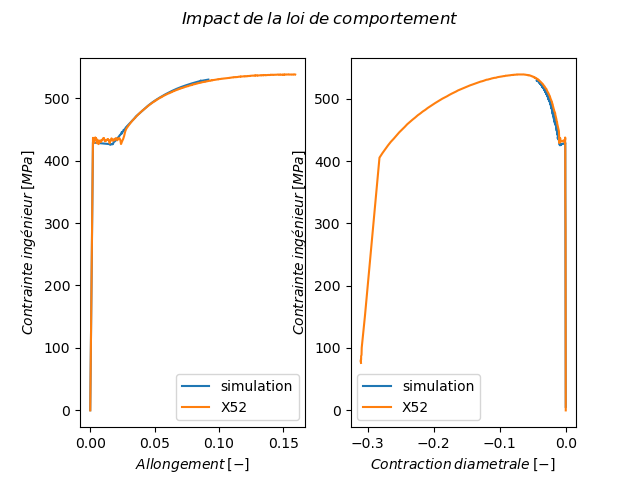
\includegraphics[width=0.6\textwidth]{image/INFLUENCE/X52_fit.png}
        \centering
        \caption{Essai de traction simulé et mesuré sur l'acier X52}
        \label{fig:X52_fit}       
    \end{figure}
    \begin{figure}[hbt]
        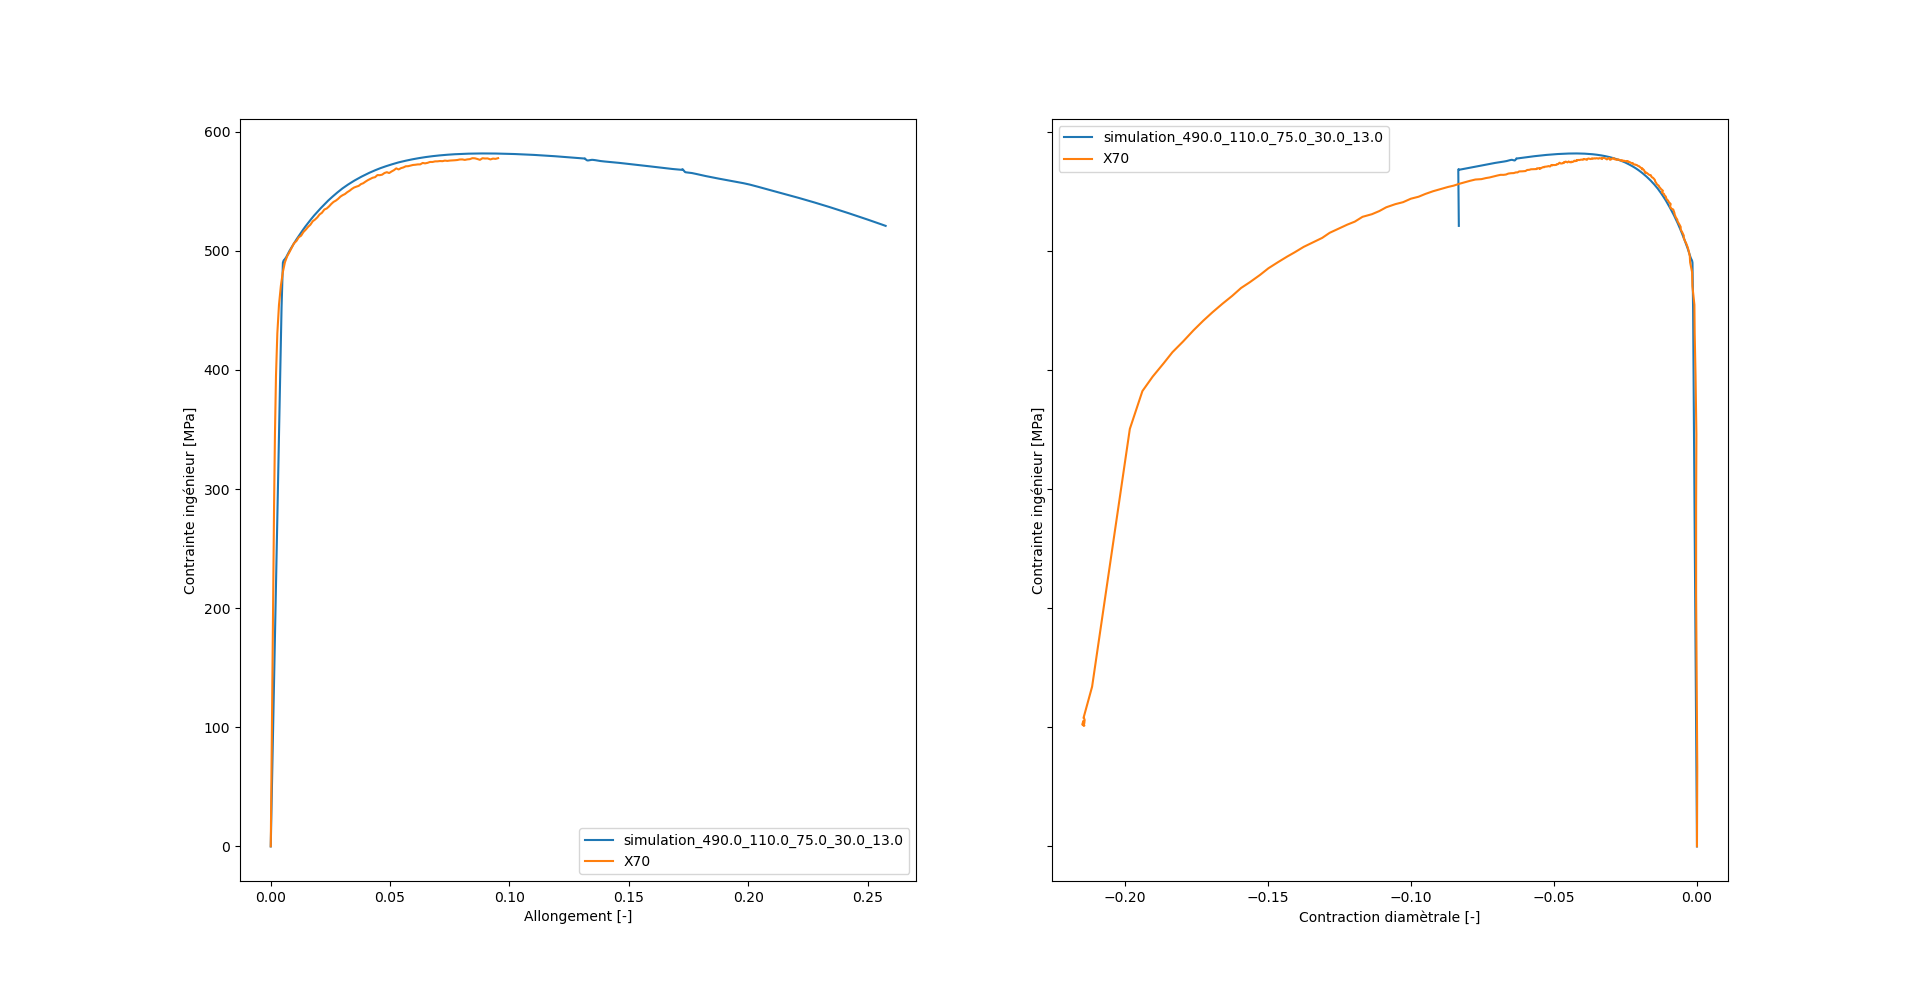
\includegraphics[width=0.6\textwidth]{image/INFLUENCE/X70_fit.png}
        \centering
        \caption{Essai de traction simulé et mesuré sur l'acier X70} 
        \label{fig:X70_fit}       
    \end{figure}

    Pour se donner une idée de l'influence des différents paramètres, on peut voir en figure \ref{fig:X52_bvar} et \ref{fig:X70_Q1var} les courbes de traction pour différentes variations des paramètres.
    
    \begin{figure}[hbt]
        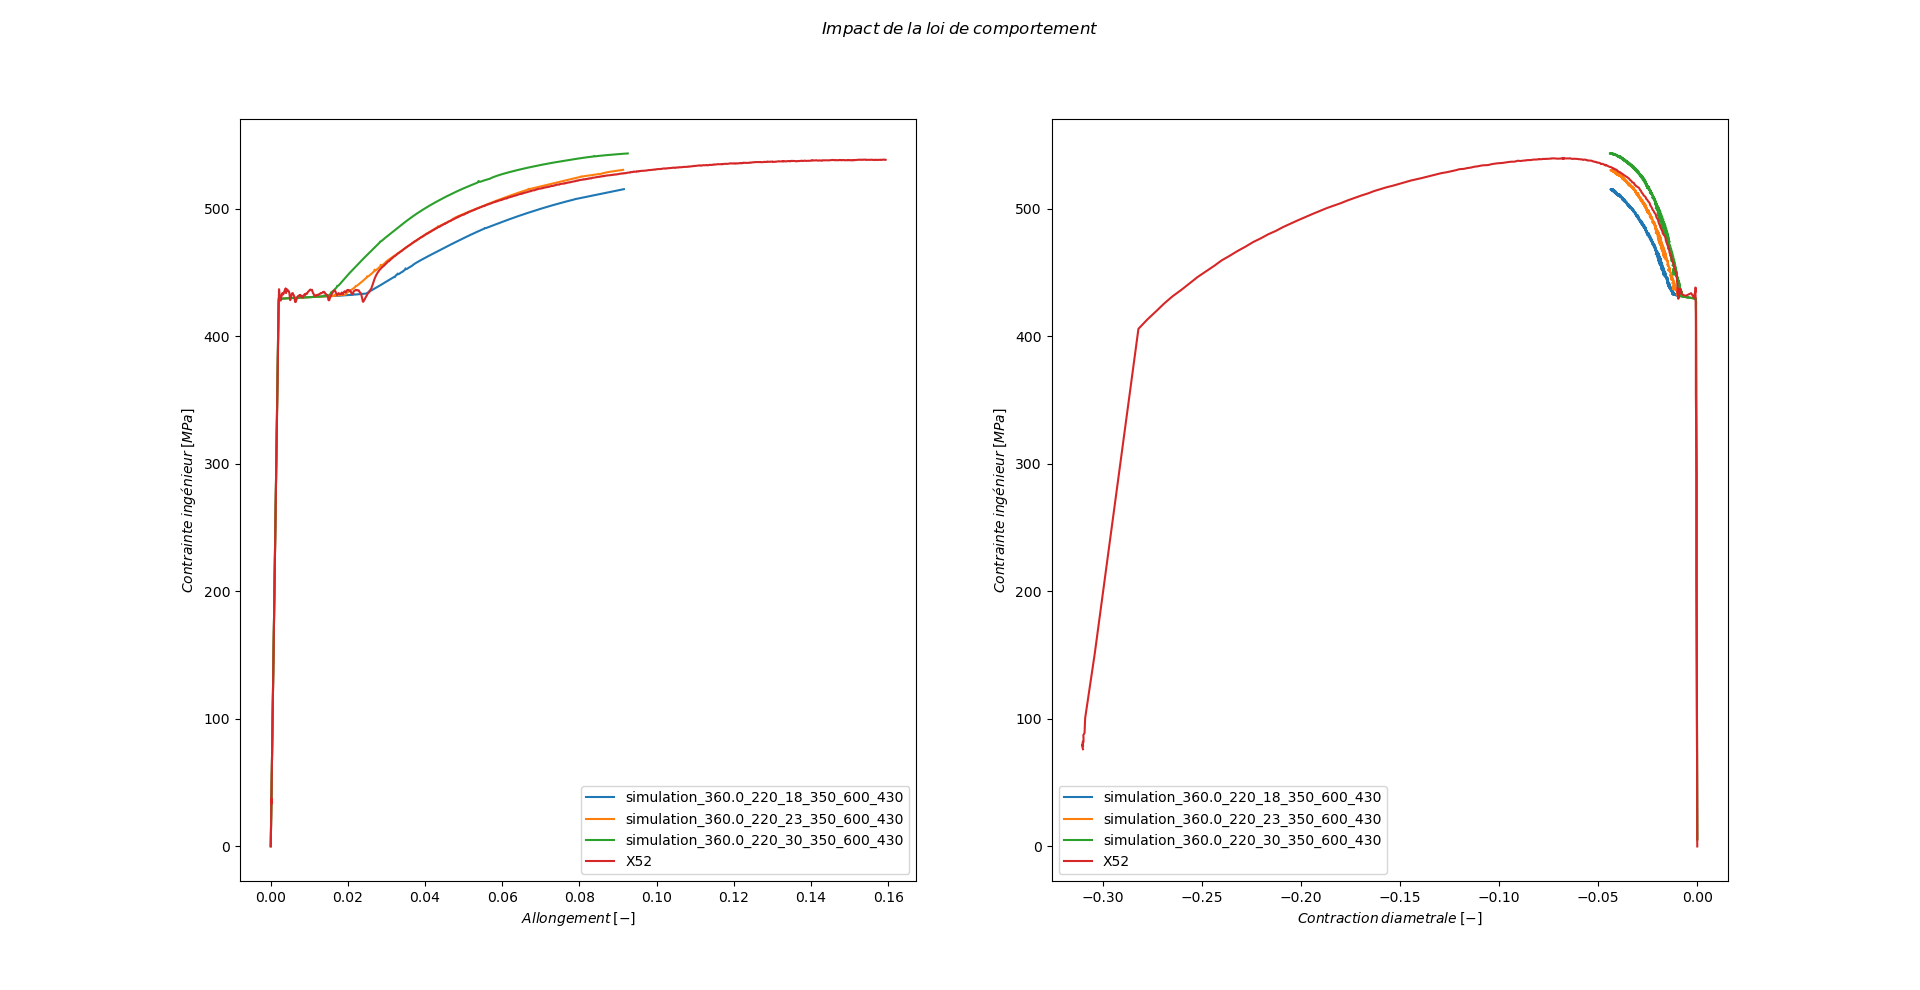
\includegraphics[width=0.6\textwidth]{image/INFLUENCE/X52_b_var_18 23_30.png}
        \centering
        \caption{Influence de la variation de b sur la simulation de l'acier X70}
 
        \label{fig:X52_bvar}
    \end{figure}

    \begin{figure}[hbt]
        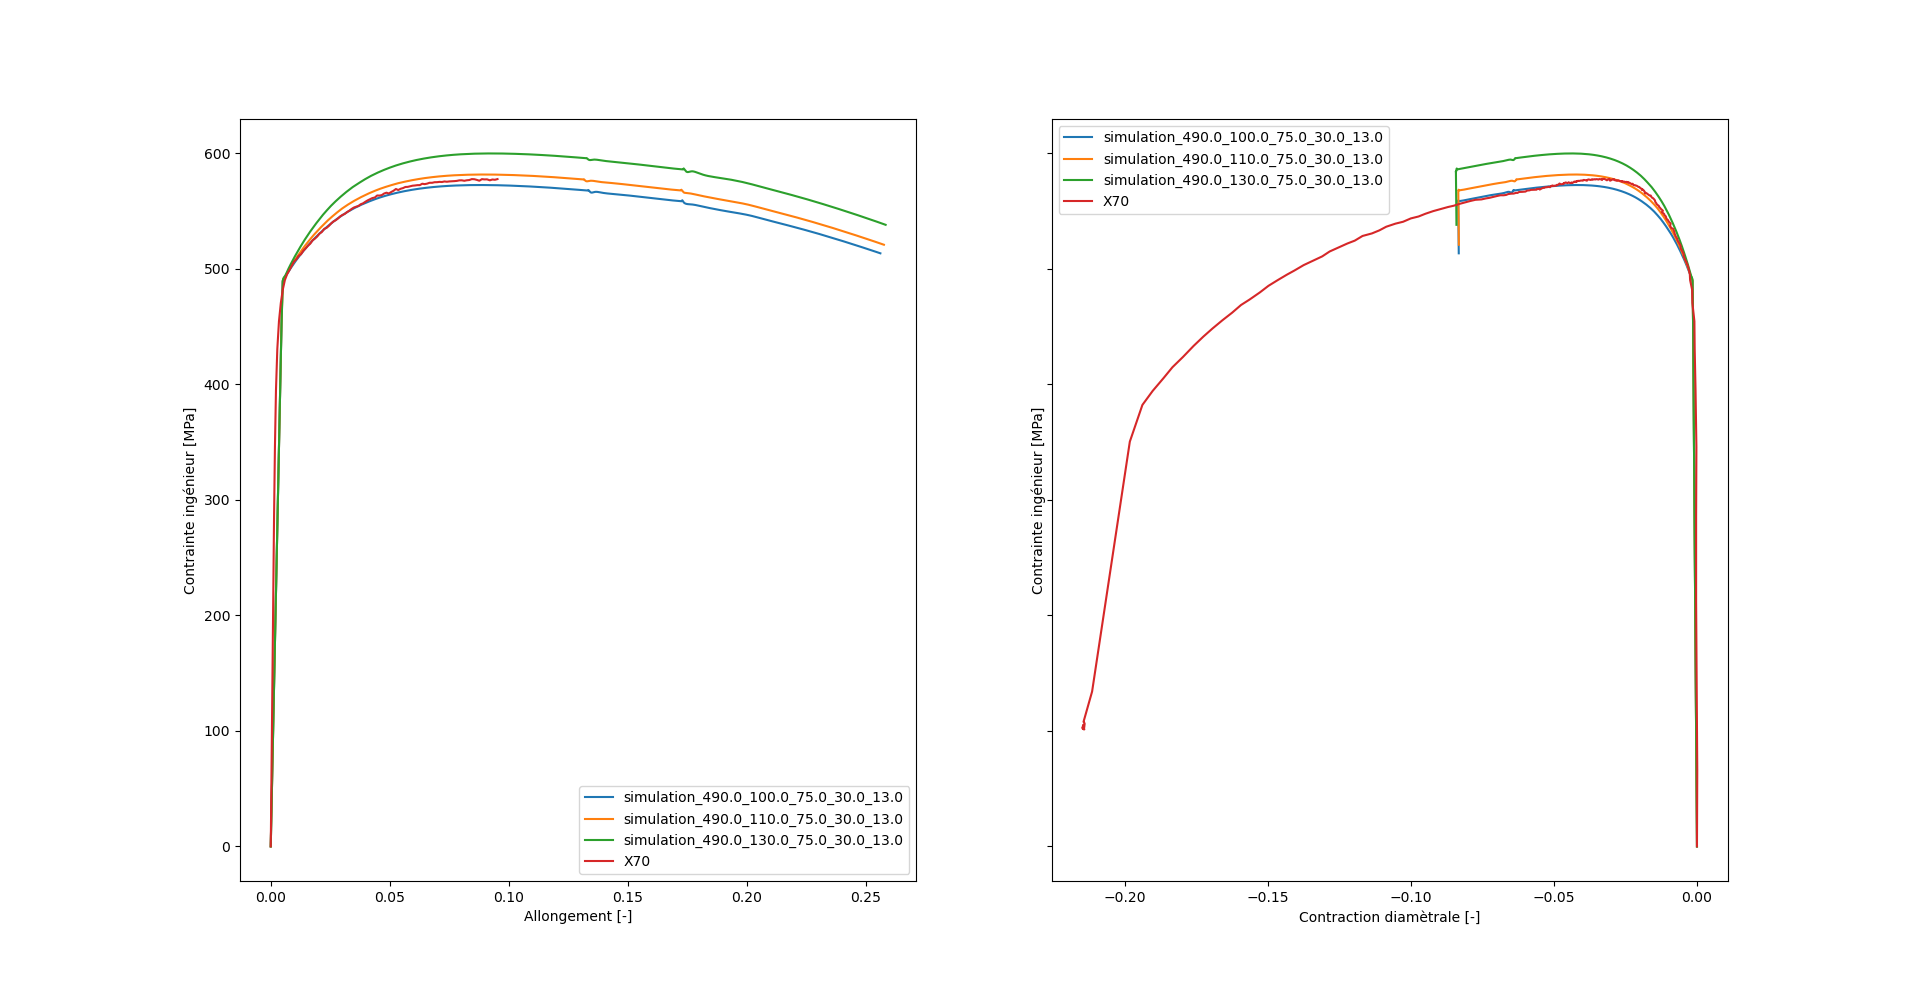
\includegraphics[width=0.6\textwidth]{image/INFLUENCE/X70_Q1_var.png}
        \centering
        \caption{Influence de la variation de Q1 sur la simulation de l'acier X70}
        \label{fig:X70_Q1var}
    \end{figure}

    Par la suite, nous avons comparé ces simulations avec les courbes expérimentales sur les éprouvettes entaillées(figures \ref{fig:X52_compar} et \ref{fig:X70_compar}), sans changer les paramètres de la loi de comportement.

    \begin{figure}[ht]
        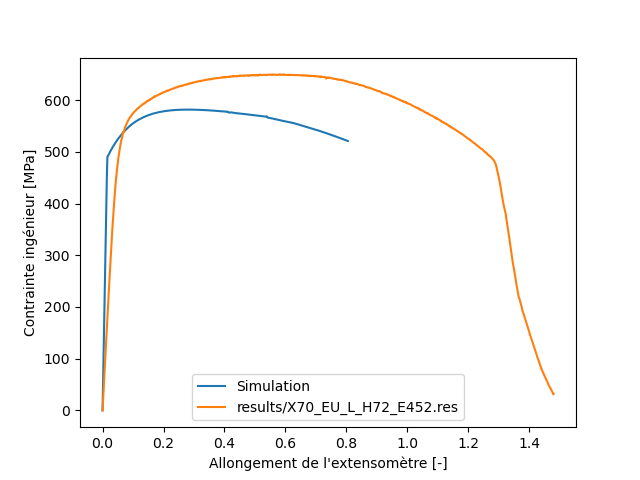
\includegraphics{image/INFLUENCE/X70_comparaison.png}
        \centering
        \caption{Comparaison simulation et expérimentation sur acier X70}
        \label{fig:X70_compar}
    \end{figure}
    
    \begin{figure}
        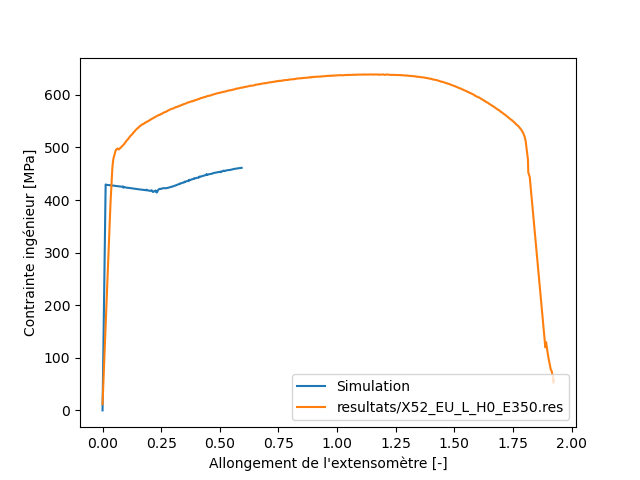
\includegraphics{image/INFLUENCE/X52_compa}
        \centering
        \caption{Comparaison simulation et expérimentation sur l'acier X52}
        \label{fig:X52_compar}
    \end{figure}
    
    La simulation continue de donner les bons ordres de grandeur, mais la prédiction des phénomènes reste assez éloigné de la réalité. Cela s'explique de plusieurs manières.
    Il existe une infinité de jeux de paramètres qui permettent de simuler les deux courbes étalons, et nous n'avons pu en tester qu'un, qui ne possède probablement pas les bonnes propriétés.
    De plus, l'hypothèse de l'indépendance de la loi de comportement par-rapport à la géométrie de la pièce, certes simplificatrice et intuitive, est peut-être trop grossière.


    \section{Implantation de l'hydrogène dans la simulation}

    \subsection{Mécanismes mis en jeu}
    L'hydrogène est présent dans l'acier grâce à deux phénomènes :
    \begin{itemize}
        \item Les aciers ayant un maillage cubique centré, et l’hydrogène pouvant se mettre dans les sites interstitiels
        \footnote{ Malgré des arguments en faveur de l'occupation des sites tétraédriques \cite{sturges_interaction_1969}, un consensus s'est établit autour de la question de l'occupation des sites intersticiels \cite{sofronis_numerical_1989}, seuls les sites octaédriques sont supposés occupés.}
         du fait de la taille faible de  ces atomes (octaédriques et tétraédriques), certains viennent se loger dans les sites interstitiels, ces atomes sont dit « libres » et peuvent se déplacer librement dans le réseau en fonction du gradient de pression. Lorsqu’une région est en compression, le maillage du réseau de fer « se resserre » et à tendance à chasser l’hydrogène. A l’inverse lorsqu’une zone voit le maillage « se dilater » elle est donc à forte pression\footnote{La convention est prise d'une normale dirigée vers "l'extérieur", une compression correspond donc à une pression négative.}, l’hydrogène va avoir tendance à s’y loger. La concentration en hydrogène à tendance à être max dans les régions de fortes pressions \cite{degtyarenko_simulation_2016}.
        \item Les défauts du réseau de fer peuvent être ponctuels ou linéaires, appelés alors dislocations. Les dislocations agissent comme des pièges à hydrogène. Comme la densité de dislocation (longueur de dislocations par unité de volume du cristal) à tendance à croître dans le domaine de déformation plastique, la densité d’hydrogène piégé est maximale là où la déformation plastique cumulée est maximale\cite{oriani_diffusion_1970}.
    \end{itemize}
    Par ailleurs, on observe des phénomènes de "pompage" de l'hydrogène libre par l'hydrogène piégé, en d'autres termes la concentration en hydrogène libre va diminuer à faveur de la concentration en hydrogène. Liée au fur et à mesure de la déformation plastique. En effet, l'ensemble des dislocations, appelée "forêt de dislocations" agis comme une "nasse" à hydrogène libre qui est piégé dans ses défauts.

    \subsection{Hypothèses et implémentation du modèle}

    Voici à présent une courte mise en équation de certains de ces concepts [(Sofronis \& McMeeking, 1989)]. 
    Nous ne prenons pas en compte l'effet de pompage de l'hydrogène libre par l'hydrogène libre.
    Notons \(C_{T}\) et \(C_{L}\) les concentrations en hydrogène libre et piégé (la concentration totale en hydrogène \(C\) est donnée par \[C = C_{T} + C_{L}\].
    On a alors : 

    \[C_{L} = \theta_{L} \beta N_{L}\]
    \[C_{T} = \theta_{T} \chi N_{T}\]

    Où \(C_{L}\) et \(C_{L}\) représentent les ratios de sites occupés sur ceux disponibles, \(C_{L} = 6\) le nombre de sites interstitiels (octaédriques seulement) disponibles par maille, \(C_{L} = 1\) le nombre d'atome d'hydrogène par piège, \(C_{L} = \) le nombre d'atomes de fer -qui constitue ici le solvant- par unité de volume et finalement \(C_{L}\) le nombre de piège par unité de volume.

    Les concentrations en hydrogène libre et piégé s'équilibrent comme suit : 
    \[K = \frac{1 - \theta_{L}}{\theta_{L}} \cdot \frac{\theta_{T}}{1-\theta_{T}}\]
    Avec:
    \[K = exp(-\frac{\boldsymbol{\Delta}E}{RT})\]
    Où  \(K\) est la constante d'équilibre associée à cette réaction d'équilibrage et \(E\) est l'énergie de l'état lié (naturellement négative). 

    
    L'équation qui régit la diffusion de l'hydrogène dans l'acier est une loi de Fick modifiée par l'ajout d'une terme en \(\nabla(V_{H}P)\) :
    \[\textbf{J}=-D\boldsymbol{\nabla}C_{L}+\frac{DC_{L}}{RT}\boldsymbol{\nabla}(V_{H}P)\]
    Où \(\textbf{J}\) est le flux d'hydrogène, \(V_{H} = 2,0 \cdot 10^{6} m^{3} \cdot mol^{-1}\) est le volume molaire partiel de l'hydrogène en solution solide, \(R = 8,314 J \cdot mol^{-1} \cdot K^{-1} \), \(P\) est la pression et \(D\) le coefficient de diffusion donné par : 
    \[D = 2 \cdot 10^{-7} e^{- 	\frac{6.88kJ \cdot mol^{-1} }{RT}	}m^{2} 		\cdot s^{-1} \]    

    On observe la concurrence de deux effets :
    \begin{itemize}
        \item comme pour une loi de diffusion classique, le terme en \((-D \nabla C_{L})\) dirige reflux vers les zones de plus faible densité d'hydrogène libre.
        \item le terme en \((+ \frac{D C_{L}}{RT} \nabla(V_{H}P))\) a quant à lui pour effet de diriger le flux vers les zones de forte pression et donc de concentrer l'hydrogène.
    \end{itemize}
    Dans nos simulations, le second effet va prendre le pas sur le premier -qui à tendance à homogénéiser la concentration en hydrogène libre- et faire ainsi apparaître des inhomogénéités dans la concentration en hydrogène libre.

    \subsection{Critères d'influence}
    La suite de l'étude portera sur les différents facteurs influant la diffusion de l'hydrogène.

    \subsubsection{Vitesse de traction}
    La diffusion de l'hydrogène dans l'acier n'est pas un phénomène instantané. En particulier, on peut mettre en évidence un temps caractéristique qui correspond au temps de diffusion de l'hydrogène sur une longueur caractéristique;
    l'hydrogène migre des zones de plus faibles pressions vers les zones de plus fortes pressions, on prend donc comme distance caractéristique de diffusion la distance entre la zone de plus faible pression et de plus faible pression.

    %include image pression cercles

    Sur cette image, on peut voir que la distance caractéristique est en ordre de grandeur la largeur de l'éprouvette. Cette approximation ne dépend pas de la vitesse de traction, on peut donc prendre comme distance caractéristique \(d = 1mm\). On a alors \[V_{diff} = \frac{D}{d} \qquad A.N. : V_{diff} = 1.10^{-6}m \cdot s^{-1}\]
    Qualitativement, on peut s'attendre à ce que \(V_{diff}\) représente une vitesse de sollicitation \nuance{palier} vis-à-vis de la diffusion de l'hydrogène; en deçà de cette vitesse, l'hydrogène a \nuance{le temps} de diffuser jusqu'à l'équilibre et au-delà de celle-ci, la concentration en hydrogène ne peut atteindre l'équilibre, le matériau est sollicité trop rapidement.
    
    \begin{figure}[ht]
        \animategraphics[autoplay, loop, width=\textwidth, controls]{5}{image/3VITESSES/step_}{000}{010}
        \centering
        \caption{Influence de la vitesse de traction sur la diffusion de l'hydrogène}
        \label{anim:3vitesse}
    \end{figure}

    On remarque l'effet annoncé, qui plus est pour une vitesse de traction proche de \(V_{diff} = 1.10^{-6}m \cdot s^{-1}\). Dès lors, la vitesse de sollicitation apparaît comme un facteur important dans l'évaluation de la faisabilité de l'injection dans le réseau de gaz naturel d'hydrogène, un gazoduc de ce réseau se dilatant naturellement suivant la demande de gaz.
    \subsubsection{Concentration initiale}

    Nous allons à présent évaluer l'influence de la concentration initiale en hydrogène sur la diffusion de ce dernier.
    Tout d'abord, il est judicieux de remarquer que selon les équations présentées plus haut et qui sont linéaires en la concentration, multiplier par un certain facteur la concentration initiale devrait avoir comme effet de multiplier par ce même facteur la concentration en tout point et à tout instant la concentration en hydrogène dans le matériau.
    Pour tester ce raisonnement, nous avons réalisé des simulations pour 3 décades de concentrations, et ce pour 2 vitesses de traction -l'une en dessous de la vitesse \(V_{diff}\) présentée plus haut et l'autre au-dessus.

    \begin{figure}[ht]
        \animategraphics[autoplay, loop, controls, width=0.8\textwidth]{5}{image/CONCENTRATIONe-5/MOVIE/step_}{000}{010}
        \caption{Vitesse de traction de \(1,0.10^{-5}\:m^2.s^{-1}\) }
    \end{figure}    

    \begin{figure}[ht]
        \animategraphics[autoplay, loop, controls, width=0.8\textwidth]{5}{image/CONCENTRATIONe-7/MOVIE/step_}{000}{010}
        \caption{Vitesse de traction \(1,0.10^{-7}\:m^2.s^{-1}\) }
    \end{figure}    

    Les résultats obtenus confirment les résultats annoncés précédemment, dans le cadre des hypothèses formulées et dans une plage raisonnable, la concentration initiale n'a que des effets linéaire sur l'évolution ultérieure de la concentration.
9
    \subsection{Limite de l'étude et développements futurs}

    En ne prenant pas en compte les phénomènes de rétroaction de l'hydrogène sur les caractéristiques mécaniques de nos matériaux, nous pouvons expliquer qualitativement	les phénomènes observés -rupture plus rapide avec hydrogène, influence de la vitesse de traction, etc. - mais pas les quantifier ce qui demeure la principale limite de notre étude. 

\end{document}